\documentclass[12pt, a4paper]{article}
\usepackage[utf8]{inputenc}
\usepackage{a4wide}
\usepackage{color, amssymb}
\usepackage{listings, amsmath, float}
\renewcommand{\baselinestretch}{1.5}
\setlength\parindent{24pt}
\usepackage{graphicx}
\graphicspath{ {./images/} }

\title{First Project}
\author{Odysseas Stavrou, Olga Tsirou}
\date{October 2020} 

\begin{document}
\noindent\rule{\textwidth}{1.5pt}

\begin{center}
{\bf Telecommunication Systems I} \\ 
 Report of the first project\\
 Olga Tsirou 2018030061\\
 Odysseas Stavrou 2018030199\\
 October 2020\\
 Technical University of Crete\\
 Prof.: A. P. Liavas 
\end{center}
\noindent\rule{\textwidth}{1.5pt}

Th.1
\[
\phi(t) = \left\{
\begin{array}{ll} 
\frac{1}{\sqrt{T}}, & \mbox{if}~|t|\le \frac{T}{2}\cr
0, & \mbox{else.}
\end{array} \right.
\]

\begin{enumerate}

\item[1.]
For: \[t +\frac{T}{2} < -\frac{T}{2}\Rightarrow t < -T\]
Then the convolution is equal to zero: \[R\phi\phi(t) = 0\]
\item[2.]
For: \[-\frac{T}{2} \le t + \frac{T}{2} \le \frac{T}{2} \Rightarrow -T \le t \le 0\] 
\[R\phi\phi(t) = \int_{-\frac{T}{2}}^{t + \frac{T}{2}} \phi(\tau) \cdot \phi(\tau + t)d\tau
= \int_{-\frac{T}{2}}^{t + \frac{T}{2}} \frac{1}{\sqrt{T}} \cdot \frac{1}{\sqrt{T}}d\tau = \frac{1}{T} \cdot (t + T) = \boxed{\frac{t}{T} + 1}
\]
\item[3.]
For: \[-\frac{T}{2} \le t - \frac{T}{2} \le \frac{T}{2} \Rightarrow 0 \le t \le T\]
\[R\phi\phi(t) = \int_{t-\frac{T}{2}}^{\frac{T}{2}} \phi(\tau) \cdot \phi(\tau + t)d\tau
= \frac{1}{T} \cdot (-t+T) = \boxed{1 - \frac{t}{T}}
\]
\item[4.]
For: \[t - \frac{T}{2} > \frac{T}{2} \Rightarrow t > T\]
The convolution is equal to zero:
\[R\phi\phi(t) = 0\]

\end{enumerate}
\[
R\phi\phi(t) = \left\{
\begin{array}{ll} 
1 + \frac{t}{T}, & -T \le t \le 0 \cr
1 - \frac{t}{T}, & 0\le t \le T\cr
0, & \mbox{else.}
\end{array} \right.
\]

\noindent\rule{\textwidth}{0.5pt}
Th.2
\[
\phi(t - 10) = \left\{
\begin{array}{ll} 
\frac{1}{\sqrt{T}}, & \mbox{if}~ -\frac{T}{2 }+ 10 \le t \le \frac{T}{2} + 10\cr
0, & \mbox{else.}
\end{array} \right.
\]
\begin{enumerate}
\item[1.]
\[t +\frac{T}{2} + 10 < -\frac{T}{2} + 10 \Rightarrow t < -T\]
Then the convolution is equal to zero: \[R\phi\phi(t) = 0\]
\item[2.]
\[-\frac{T}{2} + 10 \le t + \frac{T}{2} + 10 \le \frac{T}{2} + 10 \Rightarrow -T \le t \le 0\]
\[R\phi\phi(t) = \int_{-\frac{T}{2} + 10}^{t + \frac{T}{2} + 10} \phi(\tau) \cdot \phi(\tau + t)d\tau
=  \frac{1}{T} \cdot (t + T) = \boxed{\frac{t}{T} + 1}
\]
\item[3.]
\[-\frac{T}{2} + 10 \le t - \frac{T}{2} + 10 \le \frac{T}{2} + 10 \Rightarrow 0 \le t \le T\]
\[R\phi\phi(t) = \int_{t-\frac{T}{2} + 10}^{\frac{T}{2} + 10} \phi(\tau) \cdot \phi(\tau + t)d\tau
= \frac{1}{T} \cdot (-t+T) = \boxed{1 - \frac{t}{T}}
\]
\item[4.]
\[t - \frac{T}{2} + 10  > \frac{T}{2} + 10 \Rightarrow t > T\]
The convolution is equal to zero:\[R\phi\phi(t) = 0\]
\end{enumerate}

\[
R\phi\phi(t - 10) = \left\{
\begin{array}{ll} 
1 + \frac{t}{T}, & -T \le t \le 0 \cr
1 - \frac{t}{T}, & 0\le t \le T\cr
0, & \mbox{else.}
\end{array} \right.
\]

\noindent\rule{\textwidth}{.5pt}
Th.3
\[
\phi(t) = \left\{
\begin{array}{cl} 
\frac{1}{\sqrt{T}}, & \mbox{if}~0\le t< \frac{T}{2},\cr
-\frac{1}{\sqrt{T}}, & \mbox{if}~\frac{T}{2} \le t\le T, \cr
0, & \mbox{else.}
\end{array} \right.
\]
\begin{enumerate}
\item[1.]
\[T + t < 0 \Rightarrow t < -T\]\\
The convolution is equal to zero:\[R\phi\phi(t) = 0\]

\item[2.]
\[ t < T \] \\
The convolution is equal to zero:\[R\phi\phi(t) = 0\]

\item[3.]
\[0 \le T + t \le \frac{T}{2} \Rightarrow -T \le t \le -\frac{T}{2}\]
\[R\phi\phi(t) = \int_{0}^{T + t} \phi(\tau) \cdot \phi(\tau + t)d\tau = 
\int_{0}^{T + t} \frac{1}{\sqrt{T}} \cdot -\frac{1}{\sqrt{T}}d\tau =
-\frac{1}{T}(T + t) = \boxed{-1 - \frac{t}{T}}
\]

\item[4.]
\[\frac{T}{2} \le T + t \le T \Rightarrow -\frac{T}{2} \le  t \le 0\]
\[R\phi\phi(t) = \int_{0}^{T + t} \phi(\tau) \cdot \phi(\tau + t)d\tau \]
\[ = \int_{0}^{\frac{T}{2} + t} \phi(\tau) \cdot \phi(\tau + t)d\tau + \int_{\frac{T}{2} + t}^{\frac{T}{2}} \phi(\tau) \cdot \phi(\tau + t)d\tau + \int_{\frac{T}{2}}^{T + t} \phi(\tau) \cdot \phi(\tau + t)d\tau
\]
\[= \int_{0}^{\frac{T}{2} + t} \frac{1}{\sqrt{T}} \cdot \frac{1}{\sqrt{T}}d\tau+ \int_{\frac{T}{2} + t}^{\frac{T}{2}} -\frac{1}{\sqrt{T}} \cdot \frac{1}{\sqrt{T}}d\tau + \int_{\frac{T}{2}}^{T + t} -\frac{1}{\sqrt{T}} \cdot -(\frac{1}{\sqrt{T}})d\tau\]
\[= \frac{1}{T} \cdot (\frac{T}{2} + t) +\frac{t}{T} + \frac{1}{T} \cdot (\frac{T}{2} + t)\]
\[= \frac{1}{T} \cdot (T + 3t) = \boxed{1 + \frac{3t}{T}}
\]

\item[5.]
\[0 \le t \le \frac{T}{2}\]
\[ R\phi\phi(t) = \int_{t}^{\frac{T}{2}} \phi(\tau) \cdot \phi(\tau + t)d\tau + \int_{\frac{T}{2}}^{\frac{T}{2} + t} \phi(\tau) \cdot \phi(\tau + t)d\tau + \int_{\frac{T}{2} + t}^{T} \phi(\tau) \cdot \phi(\tau + t)d\tau
\]
\[= \int_{t}^{\frac{T}{2}} \frac{1}{\sqrt{T}} \cdot \frac{1}{\sqrt{T}}d\tau+ \int_{\frac{T}{2}}^{\frac{T}{2}+t} -\frac{1}{\sqrt{T}} \cdot \frac{1}{\sqrt{T}}d\tau + \int_{\frac{T}{2} + t}^{T} -\frac{1}{\sqrt{T}} \cdot -(\frac{1}{\sqrt{T}})d\tau\]
\[= \frac{1}{T} \cdot (\frac{T}{2} - t) - \frac{t}{T} + \frac{1}{T} \cdot (\frac{T}{2} - t)\]
\[= \frac{1}{T} \cdot (T - 3t) = \boxed{1 - \frac{3t}{T}}
\]

\item[6.]
\[\frac{T}{2} \le t \le T\]
\[R\phi\phi(t) = \int_{t}^{T} \phi(\tau) \cdot \phi(\tau + t)d\tau = 
\int_{t}^{T} -\frac{1}{\sqrt{T}} \cdot \frac{1}{\sqrt{T}}d\tau =
-\frac{1}{T}(T - t) = \boxed{-1 + \frac{t}{T}}
\]
\end{enumerate}
\[R\phi\phi(t) =\left\{
\begin{array}{cl} 
-1 -\frac{t}{T}, & -T \le t < -\frac{T}{2},\cr
1 + \frac{3t}{T}, & -\frac{T}{2} \le t < 0, \cr
1 - \frac{3t}{T}, & 0 \le t < \frac{T}{2},\cr
-1 + \frac{t}{T}, & \frac{T}{2} \le t < T, \cr
0, & \mbox{else.}
\end{array} \right.
\]

\noindent\rule{\textwidth}{.5pt}
\par By observing each $\phi$ function convoluted with its mirrored self, we can conclude that the more overlapped area they share with each other the higher the value of the self-similarity function $R\phi\phi$ with a maximum value of 1. 
\par Transposing $\phi$, and then finding its $R\phi\phi$ results in the same output function.

\noindent\rule{\textwidth}{.5pt}
\begin{enumerate}
\item[A.1]
By increasing the roll-off value (a), the further away the signal travels from its center, the more the amplitude is attenuated. Also, the higher the roll-off value the larger the maximum amplitude at the center of the pulse.

\item[A.2]
Plotting all 3 of them on the same plot was simple enough with the use of a 2D Matrix "phi", and a simple for loop:

\begin{lstlisting}[language=MATLAB]
    for i=1:3
        PHI_f(i,:) = fftshift(fft(phi(i,:),N));
        PHI_F(i,:) = PHI_f(i,:).*Ts;
        plot(f_axis,(abs(PHI_F)).^2);
        hold on;
    end
\end{lstlisting}

\item[A.3]
\begin{enumerate}
\item[a.] For each roll-off value, the theoretical Bandwidth ($=\frac{1+a}{2T}$)is:
\begin{enumerate}
\item[i.]
	$BW=500$, for $\phi$ with $a=0$
\item[ii.]
	$BW=750$, for $\phi$ with $a=0.5$
\item[iii.]
	$BW=1000$, for $\phi$ with $a=1.0$
\end{enumerate}


\item[b.]The most efficient pulse is the one with the shortest Bandwidth, in this case the pulse with the roll-off value of 0. It is worth noting that we define the cut-off point of each pulse.\\*
For cut-off at $c_1 = \frac{T}{10^-3}$
\begin{enumerate}
\item[i.]
	$BW=569.2$, for $\phi$ with $a=0$
\item[ii.]
	$BW=754.6$, for $\phi$ with $a=0.5$
\item[iii.]
	$BW=986.2$, for $\phi$ with $a=1.0$
\end{enumerate}

For cut-off at $c_2 = \frac{T}{10^-5}$
\begin{enumerate}
\item[i.]
	$BW=2110$, for $\phi$ with $a=0$
\item[ii.]
	$BW=1285$, for $\phi$ with $a=0.5$
\item[iii.]
	$BW=1168.5$, for $\phi$ with $a=1.0$
\end{enumerate}
After defining a second cutoff point the most efficient pulse become the one with roll-off $a=1$, due to its steepest decent.
\end{enumerate}
\end{enumerate}

\begin{figure}[H]
\centering
\noindent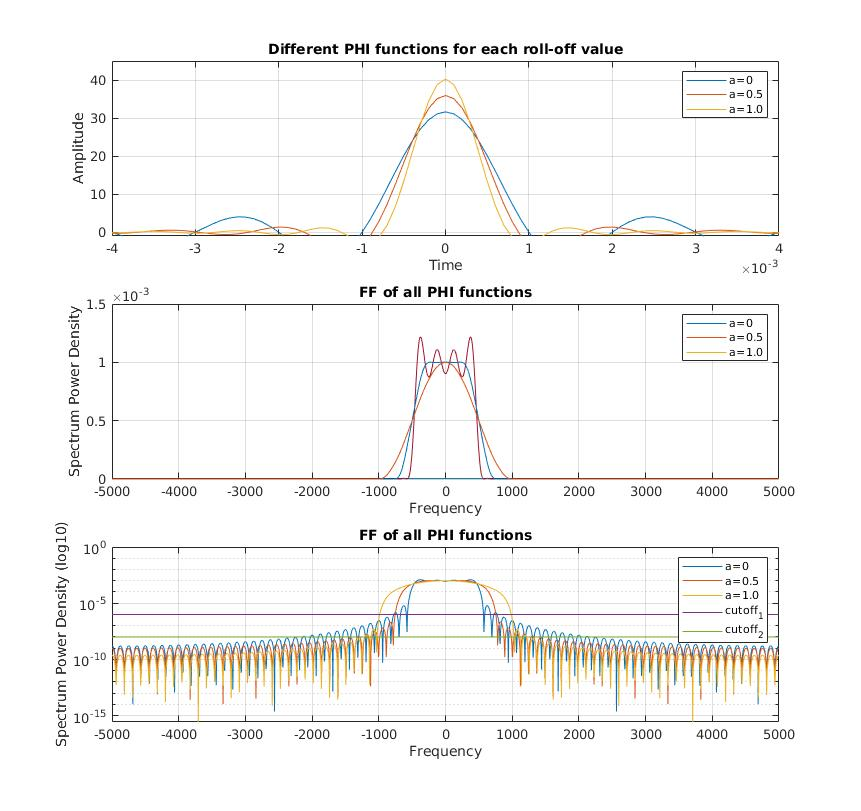
\includegraphics[width=\textwidth]{phi_ffts.jpg}
\end{figure}


\noindent\rule{\textwidth}{.5pt}
\pagebreak
\begin{enumerate}

\item[B.1] The orthocanonical function $\phi$ has some special properties. Mainly the integral with its transpositions of integer multiples of T is 0!
It is observed that the approximation of the integral gets better for $a>0$.
\begin{figure}[H]
\centering
\noindent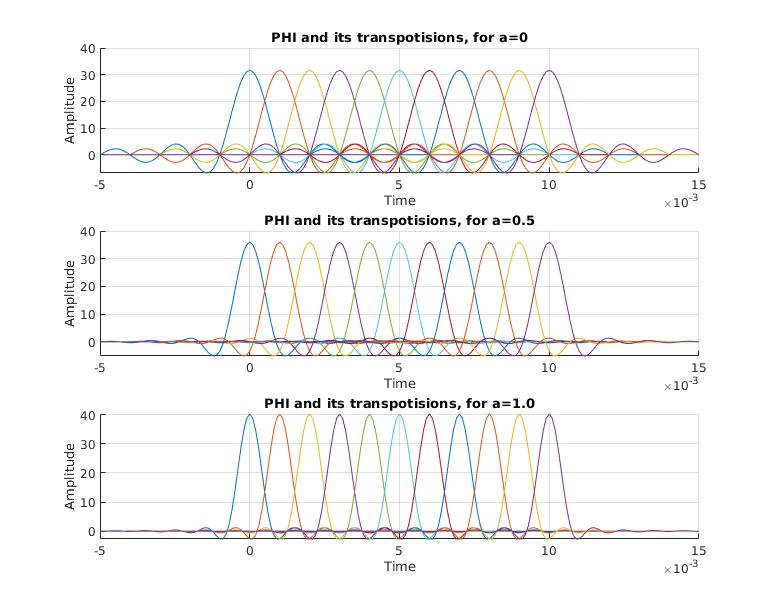
\includegraphics[width=\textwidth]{phi_k_all.jpg}
\end{figure}

\pagebreak
For $a=0$
\begin{figure}[H]
\centering
\noindent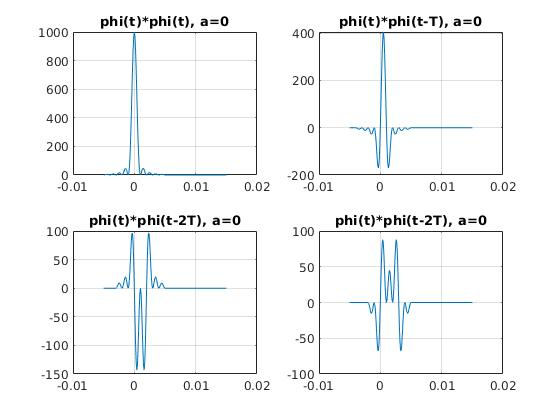
\includegraphics[width=\textwidth]{phi_k_a1.jpg}
\end{figure}
\begin{enumerate}
\item[i.] $\int_{-\infty}^{\infty} \phi(t)\phi(t) \,dt = 0.98$
\item[ii.] $\int_{-\infty}^{\infty} \phi(t)\phi(t-T) \,dt = 0.02$
\item[iii.] $\int_{-\infty}^{\infty} \phi(t)\phi(t-2T) \,dt = -0.03$
\item[iv.] $\int_{-\infty}^{\infty} \phi(t)\phi(t-3T) \,dt = 0.03$
\end{enumerate}

\pagebreak
For $a=0.5$
\begin{figure}[H]
\centering
\noindent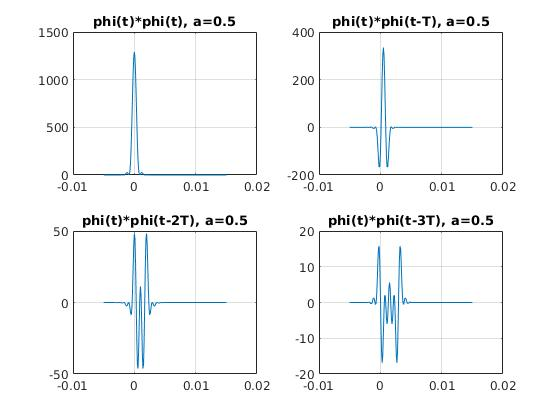
\includegraphics[width=\textwidth]{phi_k_a2.jpg}
\end{figure}
\begin{enumerate}
\item[i.] $\int_{-\infty}^{\infty} \phi(t)\phi(t) \,dt = 1$
\item[ii.] $\int_{-\infty}^{\infty} \phi(t)\phi(t-T) \,dt = 0$
\item[iii.] $\int_{-\infty}^{\infty} \phi(t)\phi(t-2T) \,dt = 0$
\item[iv.] $\int_{-\infty}^{\infty} \phi(t)\phi(t-3T) \,dt = 0$
\end{enumerate}

\pagebreak
For $a=1.0$
\begin{figure}[H]
\centering
\noindent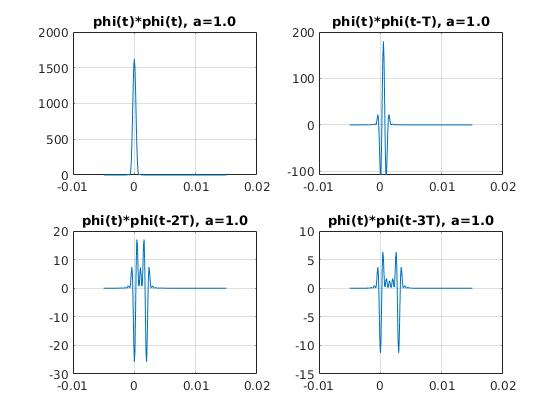
\includegraphics[width=\textwidth]{phi_k_a3.jpg}
\end{figure}
\begin{enumerate}
\item[i.] $\int_{-\infty}^{\infty} \phi(t)\phi(t) \,dt = 1$
\item[ii.] $\int_{-\infty}^{\infty} \phi(t)\phi(t-T) \,dt = 0$
\item[iii.] $\int_{-\infty}^{\infty} \phi(t)\phi(t-2T) \,dt = 0$
\item[iv.] $\int_{-\infty}^{\infty} \phi(t)\phi(t-3T) \,dt = 0$
\end{enumerate}
\end{enumerate}

\pagebreak
For creating the transpositions of $\phi(t)$ a new function called \textbf{phi\_kT} was created that returns a $length(k)$ x $length(time)$ matrix. 
It (pre)appends zeroes to $\phi(t-kT)$ so that all $\phi$'s have the same
time vector. Then the products and integrals can be computed by taking the requested rows from that matrix.
Function Code:
\begin{lstlisting}[language=MATLAB]
    function [phi_K] = phi_kT(phi, time, T, Ts, A)
        phi_K = zeros(11,length(time));
        for k=0:1:2*A
            offset = uint64(k*T/Ts);
            padL = zeros(1,offset);
            padR = zeros(1,length(time) - offset - length(phi));
            t_phi_k = [padL, phi, padR];
            phi_K(k+1,:)= t_phi_k;
        end
    end
\end{lstlisting}

\noindent\rule{\textwidth}{.5pt}



\begin{enumerate}

\item[C.1] Create N (50) random bits using the function 

\begin{lstlisting}[language=MATLAB]
    (sign(randn(bits,1)) + 1)/2
\end{lstlisting}
    	

\item[C.2] The simple 2-PAM system

\begin{enumerate}

\item[a.]The function \textbf{bits\_to\_2PAM()} maps the value of each bit to a specific symbol using the following table:
 \[0 \longrightarrow +1, \]
 \[1 \longrightarrow -1. \]
 
\pagebreak
Function Code:

\begin{lstlisting}[language=MATLAB]
    function X = bits_to_2PAM(bits)
        X = zeros(1, length(bits));
        X(bits==1) = -1;
        X(bits==0) =  1;
    end
\end{lstlisting}

\item[b.] After creating the bit stream, it gets upsampled and multiplied by $1/T_s$ so that on every sample at $kT$ a delta pulse is captured (The time vector needs readjustment to accommodate the injected zeroes): 

\begin{lstlisting}[language=MATLAB]
     X_delta = 1/Ts * upsample(X, over)
     T_delta = 0:Ts:bits/over-Ts;
\end{lstlisting}
\begin{figure}[H]
\centering
\noindent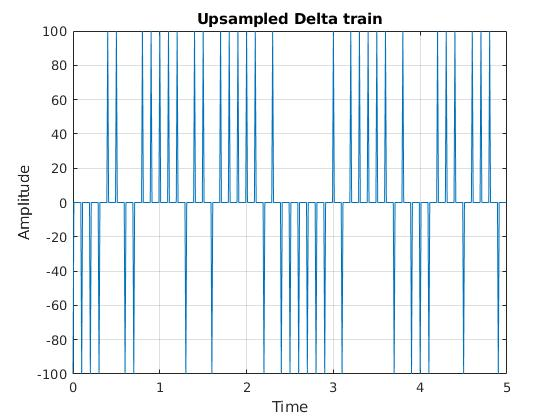
\includegraphics[width=\textwidth]{delta_train_up.jpg}
\end{figure}

\pagebreak
\item[c.] Convoluting the carrier wave $\phi(t)$ with $X\_delta$ results in the signal to be transmitted, $X(t)$:
\begin{lstlisting}[language=MATLAB]
    t_phi_conv = (t(1) + T_delta(1):Ts:t(end) + T_delta(end));
    X_t = conv(X_delta,phi)*Ts;
    plot(t_phi_conv, X_t);
\end{lstlisting}

\begin{figure}[H]
\centering
\noindent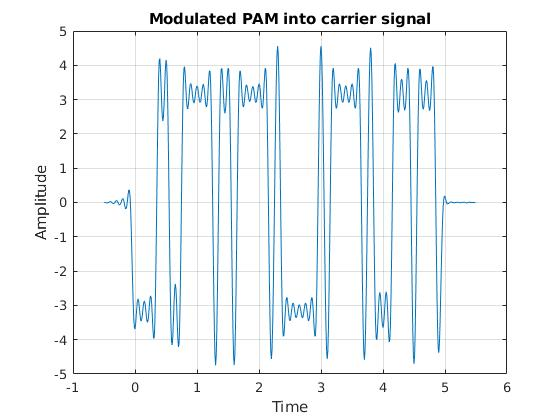
\includegraphics[width=\textwidth]{delta_pam_mod.jpg}
\end{figure}



\pagebreak
\end{enumerate}
The receiving end:
\begin{enumerate}
\item[d.] Considering an ideal communications channel, the received signal should be the $X(t)$ without any additional noise. To recreate the sequence that was sent, a convolution with the matched filter ,$\phi(-t)$, needs to be performed. The output of the filter is the integral mentioned in [B.1]. If this output is sampled at specific times it can recreate the original symbol sequence. On $kT$ multiples of $T$, $\phi$ should pass from $1$ or $-1$.
\end{enumerate}

\begin{figure}[H]
\centering
\noindent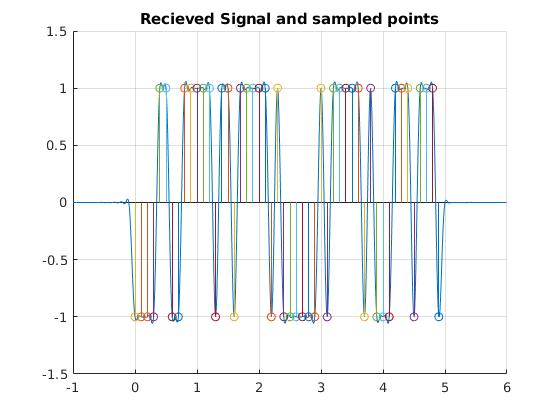
\includegraphics[width=\textwidth]{matched_filt.jpg}
\end{figure}
\pagebreak
The matched filter is created by mirroring $\phi$ and its time vector using:
\begin{lstlisting}[language=MATLAB]
    t_phi_minus = -fliplr(t);
    phi_minus = fliplr(phi);
\end{lstlisting}


After filtering, the convolution can take place and then the sampling
\begin{lstlisting}[language=MATLAB]
    tconv = (t_phi_minus(1) + t_phi_conv(1):Ts:t_phi_minus(end) +                        t_phi_conv(end));
    X_z = conv(phi_minus, X_t)*Ts;
    plot(tconv, X_z);
    stem((0:49)*T,X_50);
    for t=1:length(tconv)
       if mod(tconv(t), T) == 0 && tconv(t) >= 0 
           && tconv(t) <= A(2)-Ts
          stem(tconv(t), X_z(t)); 
       end
    end
\end{lstlisting}
\pagebreak
Looking closely one would observe that there is a slight deviation from the sent symbol and the received one. All sent symbols line up perfectly on $y=1$ and $y=-1$, however because $\phi$ is just an approximation a slight deviation is expected.
\begin{figure}[H]
\centering
\noindent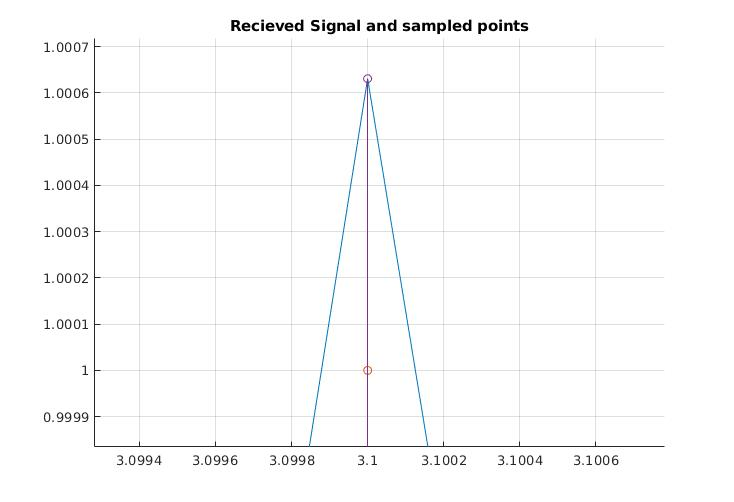
\includegraphics[width=\textwidth]{deviation.jpg}
\end{figure}
\end{enumerate}
\begin{lstlisting}[language=MATLAB]
    
    
\end{lstlisting}
\end{document}